\subsection{Caso d'uso UC3: Login}
\begin{center}
	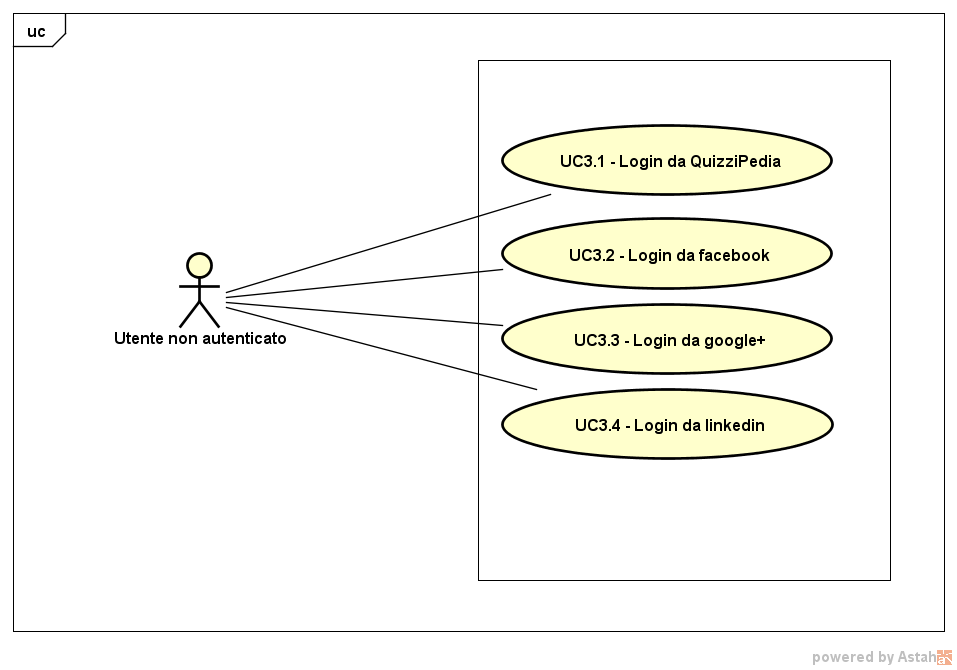
\includegraphics[scale=0.5]{UML/UC3.png}
\end{center}
\begin{itemize}
	\item \textbf{Attori}: utente non autenticato;
	\item \textbf{Descrizione}: l'attore si può autenticare: inserisce nome utente e password con cui è registrato ed effettua il login;
	\item \textbf{Precondizione}: il sistema è avviato e pronto per l'utilizzo e mostra la pagina di login;
	\item \textbf{Flusso principale degli eventi}:
	\begin{enumerate}
		\item L'attore inserisce il nome utente oppure la mail utilizzata al momento della registrazione (UC3.1);
		\item L'attore inserisce la password (UC3.2);
		\item L'attore conferma il login (UC3.3).
	\end{enumerate}
	\item \textbf{Scenario alternativo:}
	\begin{itemize}
		\item L'attore inserisce un nome utente inesistente;
		\item L'attore inserisce una mail non registrata;
		\item L'attore non inserisce ne un nome utente ne una mail;
		\item L'attore inserisce una password errata;
		\item L'attore non inserisce una password.
	\end{itemize}
	In tal caso il sistema ritorna allo stato precedente l'inserimento dei dati e viene visualizzato un messaggio d' errore.
	\item \textbf{Estensione:} l'attore visualizza un messaggio d'errore di autenticazione (UC3.4).
	\item \textbf{Postcondizione:} il sistema ha autenticato l'attore e quindi mostra all'attore autenticato la sua area riservata.
\end{itemize}

\subsubsection{Caso d'uso UC3.1: inserimento del nome utente o della mail}
\begin{itemize}
	\item \textbf{Attori}: utente;
	\item \textbf{Descrizione}: l'attore inserisce il proprio nome utente creato oppure la mail utilizzata al momento della registrazione [UC2];
	\item \textbf{Precondizione}: il sistema presente all'attore lo spazio destinato a questa operazione;
	\item \textbf{Postcondizione}: il nome utente è stato inserito.
\end{itemize}
\subsubsection{Caso d'uso UC3.2: inserimento della password}
\begin{itemize}
	\item \textbf{Attori}: utente;
	\item \textbf{Descrizione}: l'attore inserisce la propria password associata al proprio nome utente creata al momento della registrazione (UC2);
	\item \textbf{Precondizione}: il sistema presenta all'attore lo spazio destinato a questa operazione;
	\item \textbf{Postcondizione}: la password associata al nome utente è stata inserita.
\end{itemize}
\subsubsection{Caso d'uso UC3.3: conferma login}
\begin{itemize}
	\item \textbf{Attori}: utente;
	\item \textbf{Descrizione}: l'attore conferma i dati inseriti per tentare una login;
	\item \textbf{Precondizione}: il nome utente o la mail e la password devono essere stati inseriti;
	\item \textbf{Postcondizione}: l'attore è autenticato.
\end{itemize}
\subsubsection{Caso d'uso UC3.4: visualizza errore di autenticazione}
\begin{itemize}
	\item \textbf{Attori}: utente;
	\item \textbf{Descrizione}: l'attore visualizza un errore per fallimento del tentativo di login;
	\item \textbf{Precondizione}: l'attore ha confermato il login;
	\item \textbf{Postcondizione}: l'attore visualizza il messaggio d'errore e può procedere con un nuovo inserimento del nome utente o della mail (UC3.1) o della password (UC3.2).
\end{itemize}